\documentclass[twocolumn]{article}
\usepackage{arxiv}

\usepackage[utf8]{inputenc}
\usepackage[T1]{fontenc}
\usepackage{url}
\usepackage{booktabs}
\usepackage{amsmath,amssymb,amsfonts}
\usepackage{microtype}
\usepackage{graphicx}
\usepackage{siunitx}
\usepackage{caption}
\usepackage{subcaption} 

\usepackage[numbers,square,comma,sort&compress]{natbib}

% Let columns end naturally instead of being vertically stretched to fill the
% page (\flushbottom), which otherwise inflates the glue after section headings.
\raggedbottom

\graphicspath{{./images/}{./}}

% ------------------------------------------------------------------
% Title and author
% ------------------------------------------------------------------
\title{A Unified Framework for Automated Disruption Labeling of DIII-D shots using a 1D Convolutional Neural Network and Temporal Filtering}

\author{
  Jason Jain, Jesse A. Rodríguez \\
  School of Mechanical, Industrial, and Manufacturing Engineering \\
  Oregon State University \\
  Corvallis, OR 97331, USA \\
  \texttt{jainsp@oregonstate.edu}, \texttt{jesse.rodriguez@oregonstate.edu}
}

\begin{document}

\twocolumn[
  \maketitle
  \begin{@twocolumnfalse}
    \begin{abstract}
    Plasma in a Tokamak fusion reactor frequently experiences disruption events that result in a current drop to zero. The existence of a computationally inexpensive model for identifying disruptive shots and accurately identifying time of disruption can assist the scientific community by auto-labeling shots for further analysis. We took a labeled disruption dataset from the DIII-D Tokamak reactor, utilizing shot numbers 125500-186000 (nearly 40,000 total shots) to develop a new disruption labeling model that can generate automated labeling up to the current day. We train a CNN (Convolutional Neural Network) to perform boolean disruption/not-disruption prediction and achieve a 99\% recall and 91\% precision on our test dataset. We additionally develop a convolutional heuristic that accurately identifies time of disruption with a median of $0$ and standard deviation of $\qty{1.1}{\milli\s}$.
    \end{abstract}
    \vspace{1em}
  \end{@twocolumnfalse}
]


% ==================================================================
\section{Introduction}
\label{sec:intro}
A Tokamak is a torus-shaped magnetic confinement fusion reactor and is a leading candidate to produce controlled thermonuclear fusion power. A prominent challenge facing Tokamak reactors is the issue of disruption events caused by turbulent instability within the plasma. Such disruption events cause the internal reactor current ($I(t)$) to drop to zero and can potentially cause damage to the interior of the reactor \cite{egemen2023}. The differential equations describing the evolution of such turbulent plasma are not solvable with conventional numerical methods; therefore, deep learning models trained on labeled plasma data are a promising approach for predicting such disruptions before they happen.

A fraction of the data produced by long-running Tokamak fusion facilities such as the DIII-D reactor in Argonne National Laboratory have already been labeled for training of such models. We used nearly 40,000 DIII-D shots to train a model for labeling historical shots as disruptive or not disruptive. We also develop a convolutional heuristic for identifying a time of disruption that closely matches the labeled DIII-D disruption times.

% ==================================================================
\section{Neural Net Classifier}
\label{sec:methods}


We were provided 39438 labeled shot files from the DIII-D team, of which 13429 were disruptive shots and labeled with time of disruption. Each shot sampled reactor current at $\qty{40}{\kilo\hertz}$, giving us a discrete $1 \times m$ current vector $\mathbf{I}$ where the $m$th component is current at the $m$th timestep. 

\begin{equation}
  \label{current_tensor}
  \mathbf{I}=\begin{bmatrix} I_1 & \dots & I_m \end{bmatrix}
\end{equation}

We used an 80/10/10 train/test/dev split, which left us with 31542 trainable shots. To prepare the data for a neural net classifier, we tested three different normalization methods, including per-shot min-max unit scale normalization,  per-shot Mean-Variance (meanvar) normalization, and dataset-wide meanvar normalization. We found most success with the dataset-wide meanvar approach. Letting the current mean and standard deviation across all shots be $\mu$ and $\sigma$, we computed a normalized shot tensor $I_\mathrm{N}$. 

\begin{equation}
  \label{current_norm}
\mathbf{I}_{\mathrm{N}} =
\begin{cases}
\frac{1}{\sigma}(\mathbf{I} - \mu) & \sigma > 0 \\[0.5em]
  0 & \sigma \leq 0  
\end{cases}  
\end{equation}

The normalized data was then fed into a Convolutional Neural Network (see ~Figure~\ref{fig:model_diagram}) consisting of four convolutional layers, each with a batch normalization layer, a Rectified Linear Unit (ReLU) activation function, and a final max pooling layer. The convolution outputs were then fed into two fully connected layers with batch normalization, ReLU, and a dropout layer to prevent overfitting. The dropout layer exposed a dropout rate \verb|dropout| hyperparameter. 



\begin{figure}[h]
  \centering
  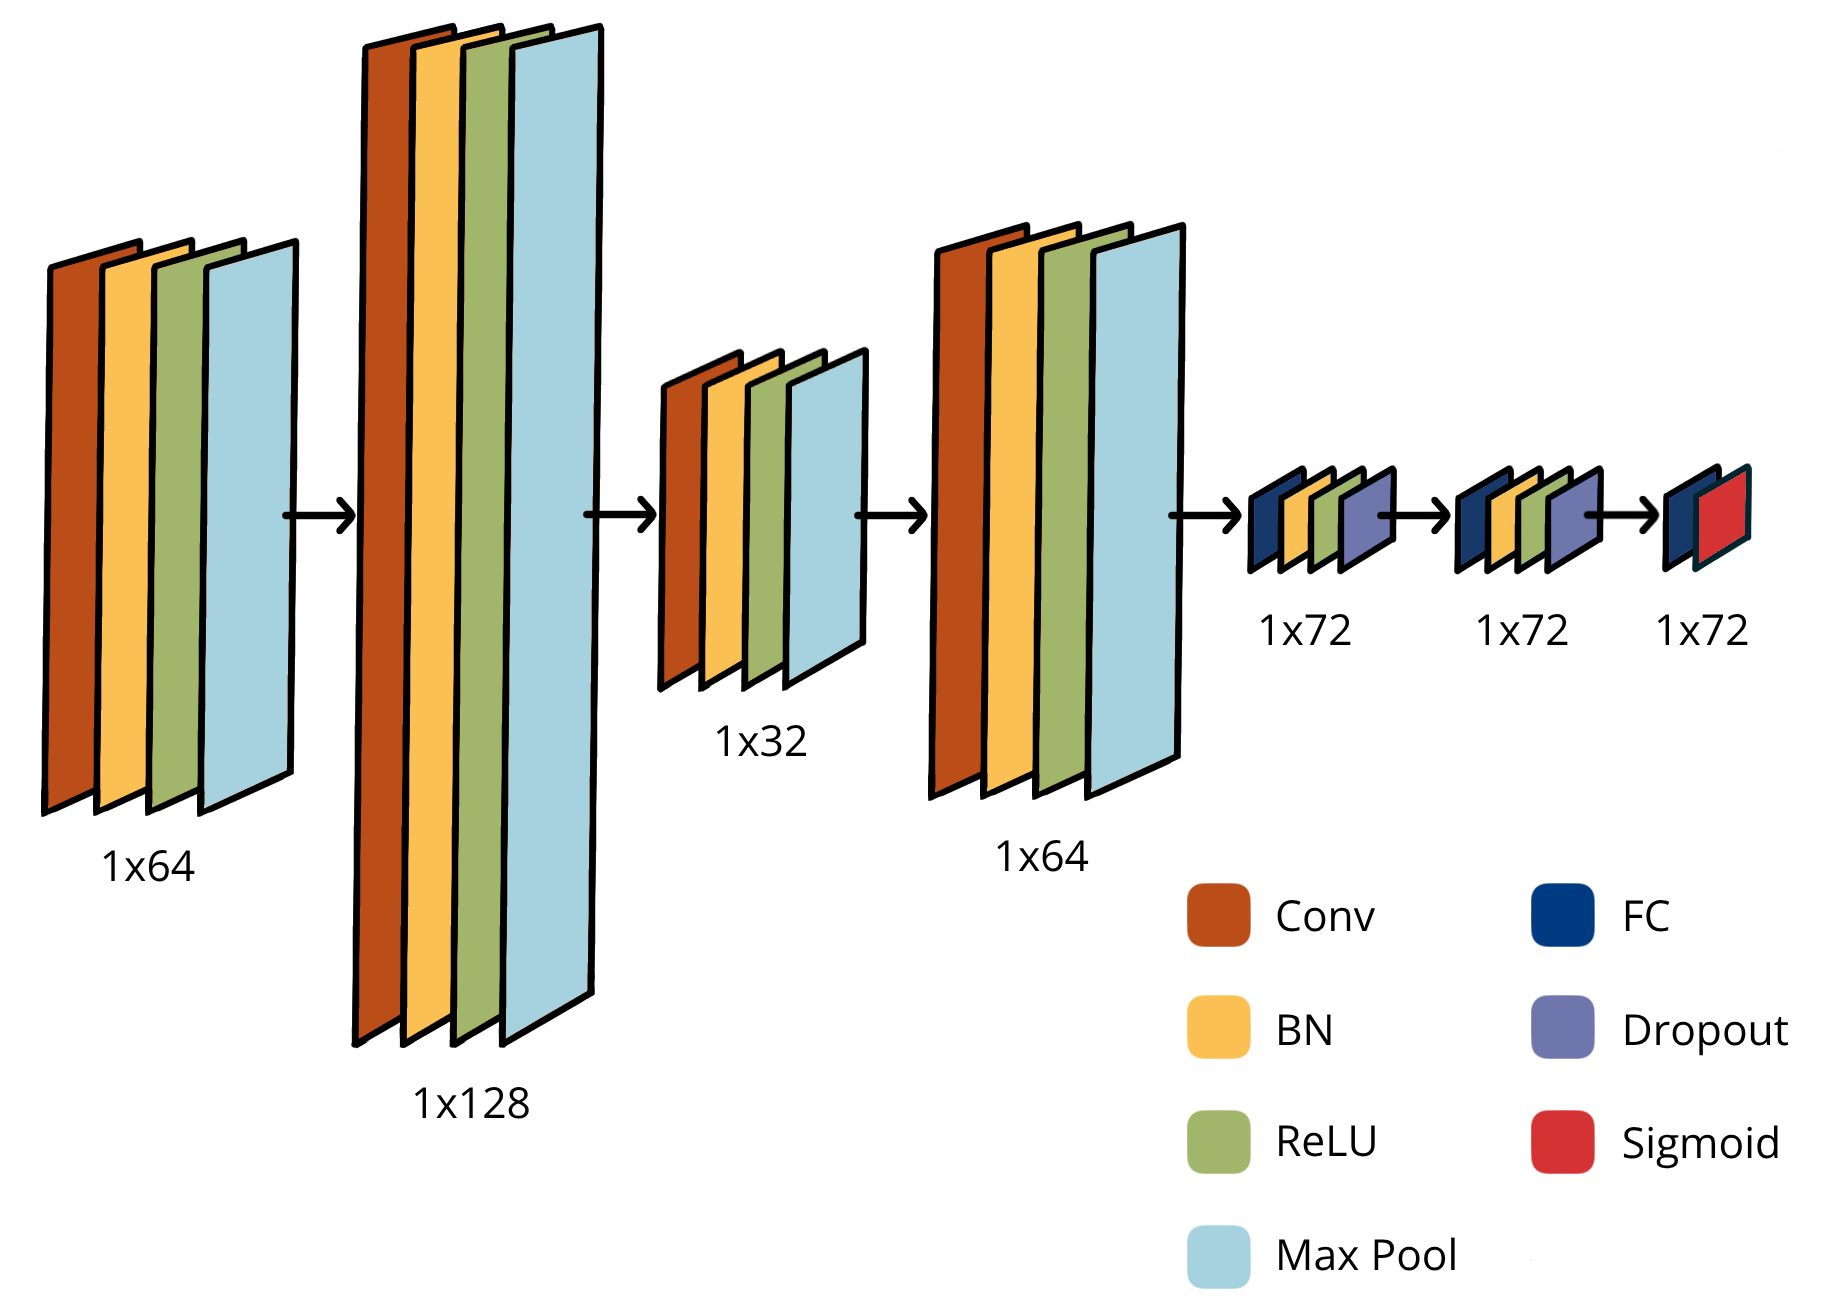
\includegraphics[width=\columnwidth]{best_model/model_diagram.png}
  \caption{Model architecture for our disruption labeling Convolutional Neural Network. We have four convolutional layers and two fully connected layers, and utilize max pooling, batch normalization, and dropout, along with a ReLU activation function. The model input is normalized current sampled at $\qty{40}{\kilo\hertz}$ and the output is disruption probability for the shot. }
  \label{fig:model_diagram}
\end{figure}



The CNN was then trained using the Adam (Adaptive Moment Estimation) optimizer with weight decay and a learning rate tuned per-epoch with PyTorch's \verb|lr_scheduler.ReduceLROnPlateau| in "min" mode, with configurable learning rate factor and patience. We utilized PyTorch's \verb|torch.nn.BCEWithLogitsLoss| with configurable positive weight and gradient clipping, and stopped training when enough consecutive epochs showed no improvement (early stopping patience).

We tuned our hyperparameters with Bayesian Optimization, using the \verb|ExpectedImprovement| acquisition function with $\xi=0.05$. We additionally inserted random samples every 5 trials to escape local minima. Our scoring strategy was a weighted $F_\beta$, where parameter $\beta$ is the weighted harmonic mean of precision and recall (Eq~\eqref{fbeta}). We chose $\beta=1.5$ to prioritize recall ($R$) over precision ($P$) and minimize false negatives, rejecting trials below a precision floor of 90\%. 


\begin{equation}
  \label{fbeta}
  F_\beta =  \frac{PR(1 + \beta^2)}{P\beta^2+R}
\end{equation}

We trained for 100+ trials on the Polaris supercomputer in Argonne National Lab, achieving a final precision of 90.52\% and recall of 98.84\%, along with an F1 score of $0.9450$ and F2 score of $0.9706$. The tuned hyperparameters are presented in ~\ref{tab:hyperparams}. 
          
\begin{table}[h]
    \centering
    \caption{Tuned Hyperparameters}
    \label{tab:hyperparams}
    \begin{tabular}{|l|r|}
        \hline
        \textbf{Hyperparameter} & \textbf{Value} \\
        \hline
          Learning Rate & 0.0005  \\
        \hline
          Number of Epochs & 200  \\
        \hline
          Dropout Rate & 0.35  \\
        \hline
          Weight Decay & 0.0001  \\
        \hline
          Training Batch Size & 128  \\
        \hline
          Gradient Clip & 1.0  \\
        \hline
          Learning Rate Scheduler Factor  &  0.5 \\
        \hline
          Learning Rate Patience  & 5  \\
        \hline
          Early Stopping Patience & 10  \\
        \hline
          Positive Weight  & 3.0  \\
        \hline
    \end{tabular}
\end{table}



\begin{figure}[t]
  \centering
  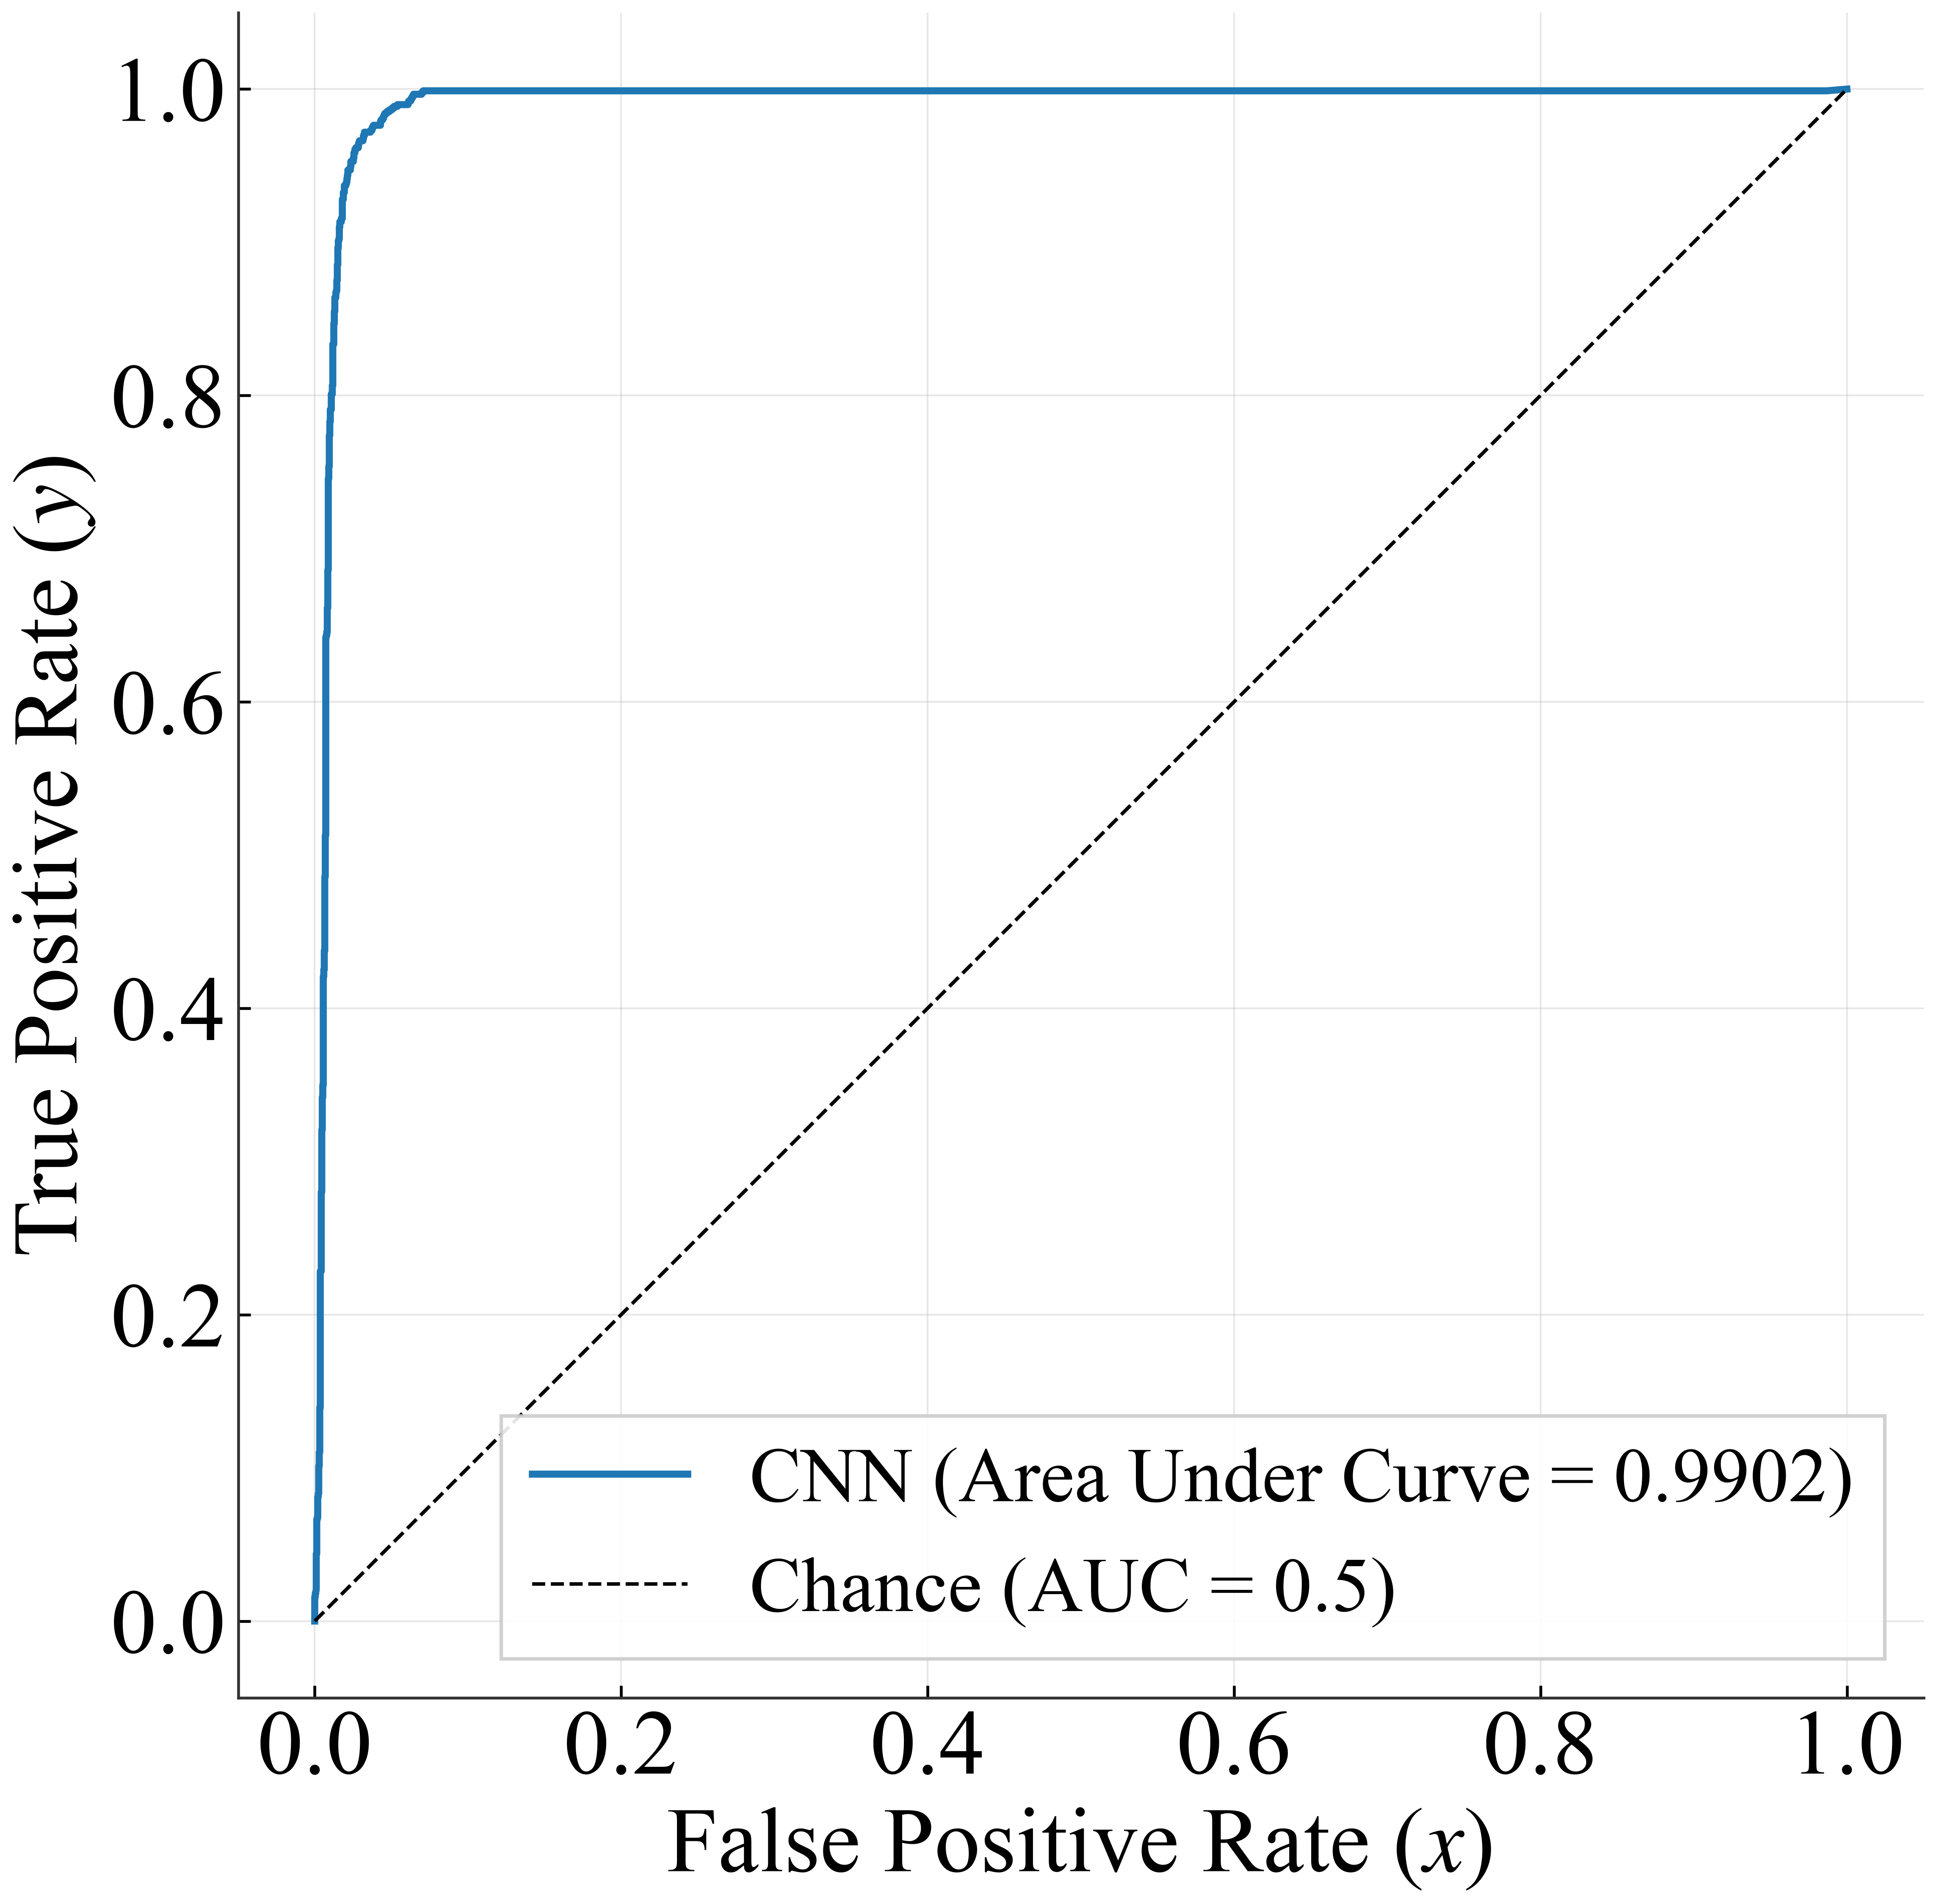
\includegraphics[width=1\columnwidth]{best_model/roc_curve.png}
  \caption{The ROC curve for our disruption classifier. The integral (AUC) of the ROC characterizes a classifier's performance, with a score of 1 indicating 100\% true positives and 0\% false negatives. Our model has an AUC of 0.9902, close to the hypothetical maximum.  }
  \label{fig:roc}
\end{figure}


The false negatives produced by the model lack the characteristic drop to zero, and some look like faulty data. See Figure~\ref{fig:cnn_errors}. 

\begin{figure*}[htp]
  \centering
  
  \begin{subfigure}[b]{0.48\textwidth}
    \centering
    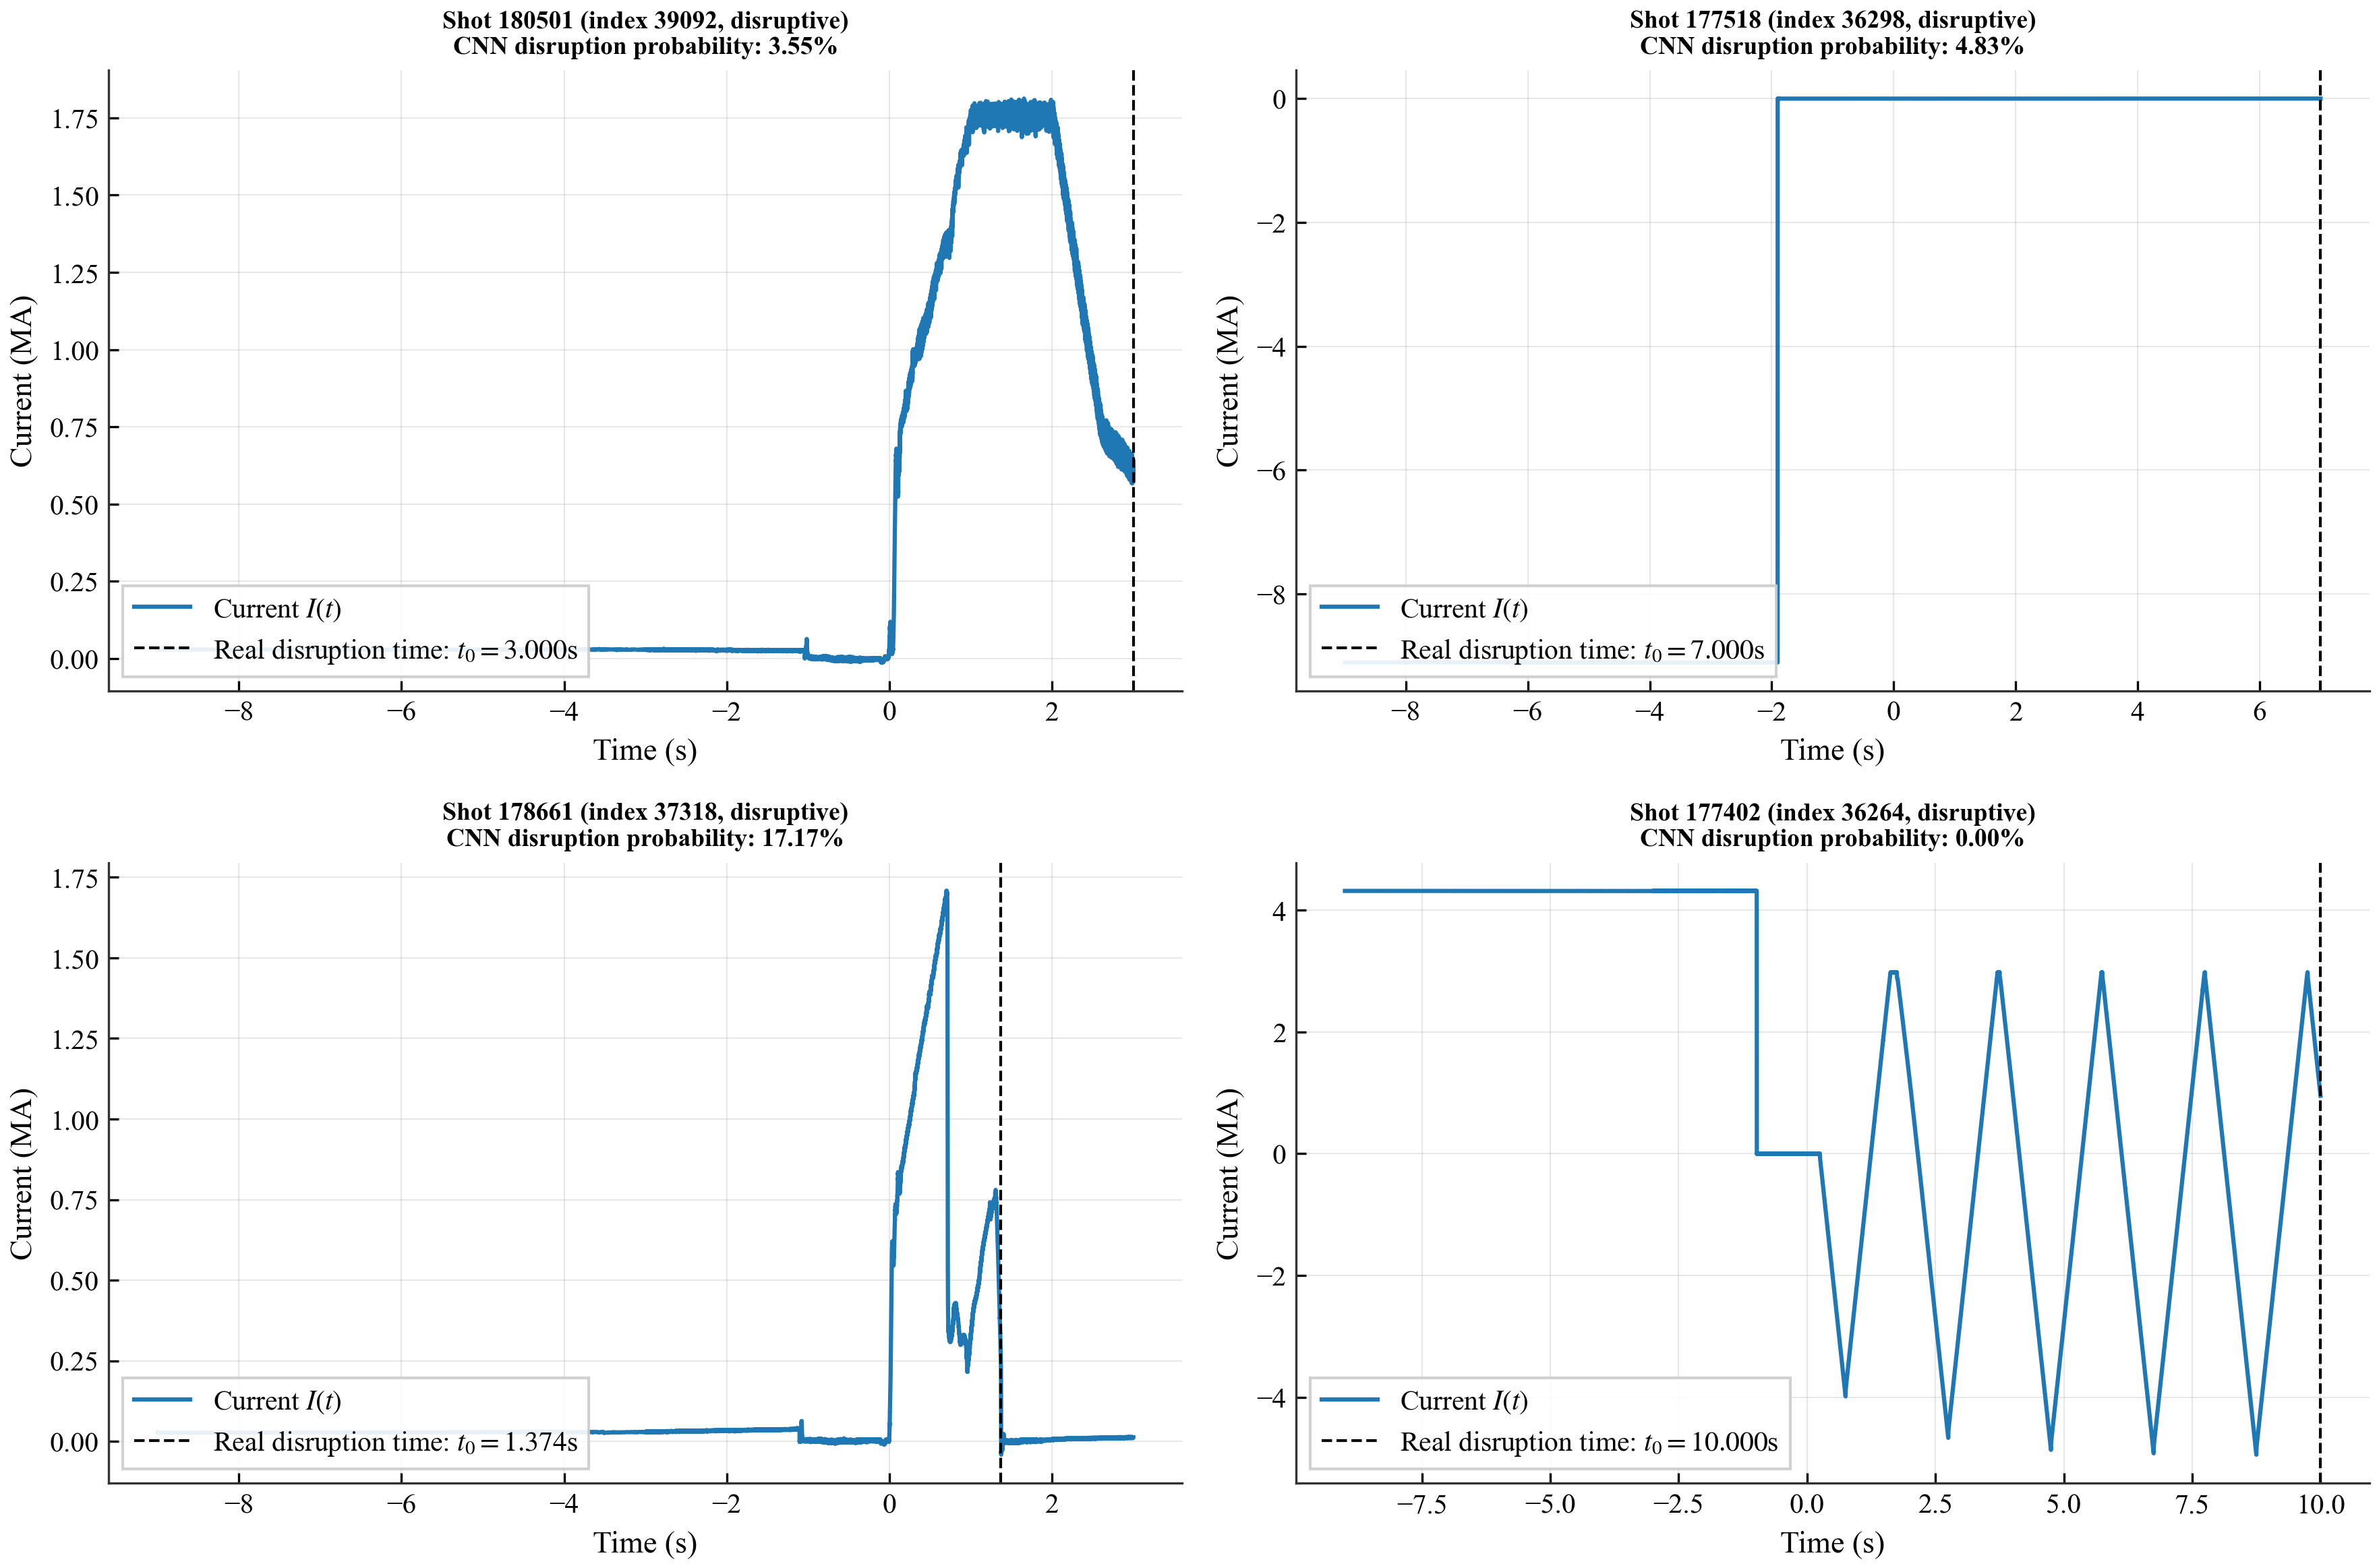
\includegraphics[width=\textwidth]{best_model/select_false_negatives.png}
    \caption{Four selected disruptive shots incorrectly identified as non-disruptive by the CNN. Each shot lacks the characteristic instant drop to zero that typically identifies a disruption. Shots 180501 and 177403 read like faulty data, as if the device stopped recording mid-experiment.}
    \label{sub:false_negatives}
  \end{subfigure}
  \hfill
  \begin{subfigure}[b]{0.48\textwidth}
    \centering
    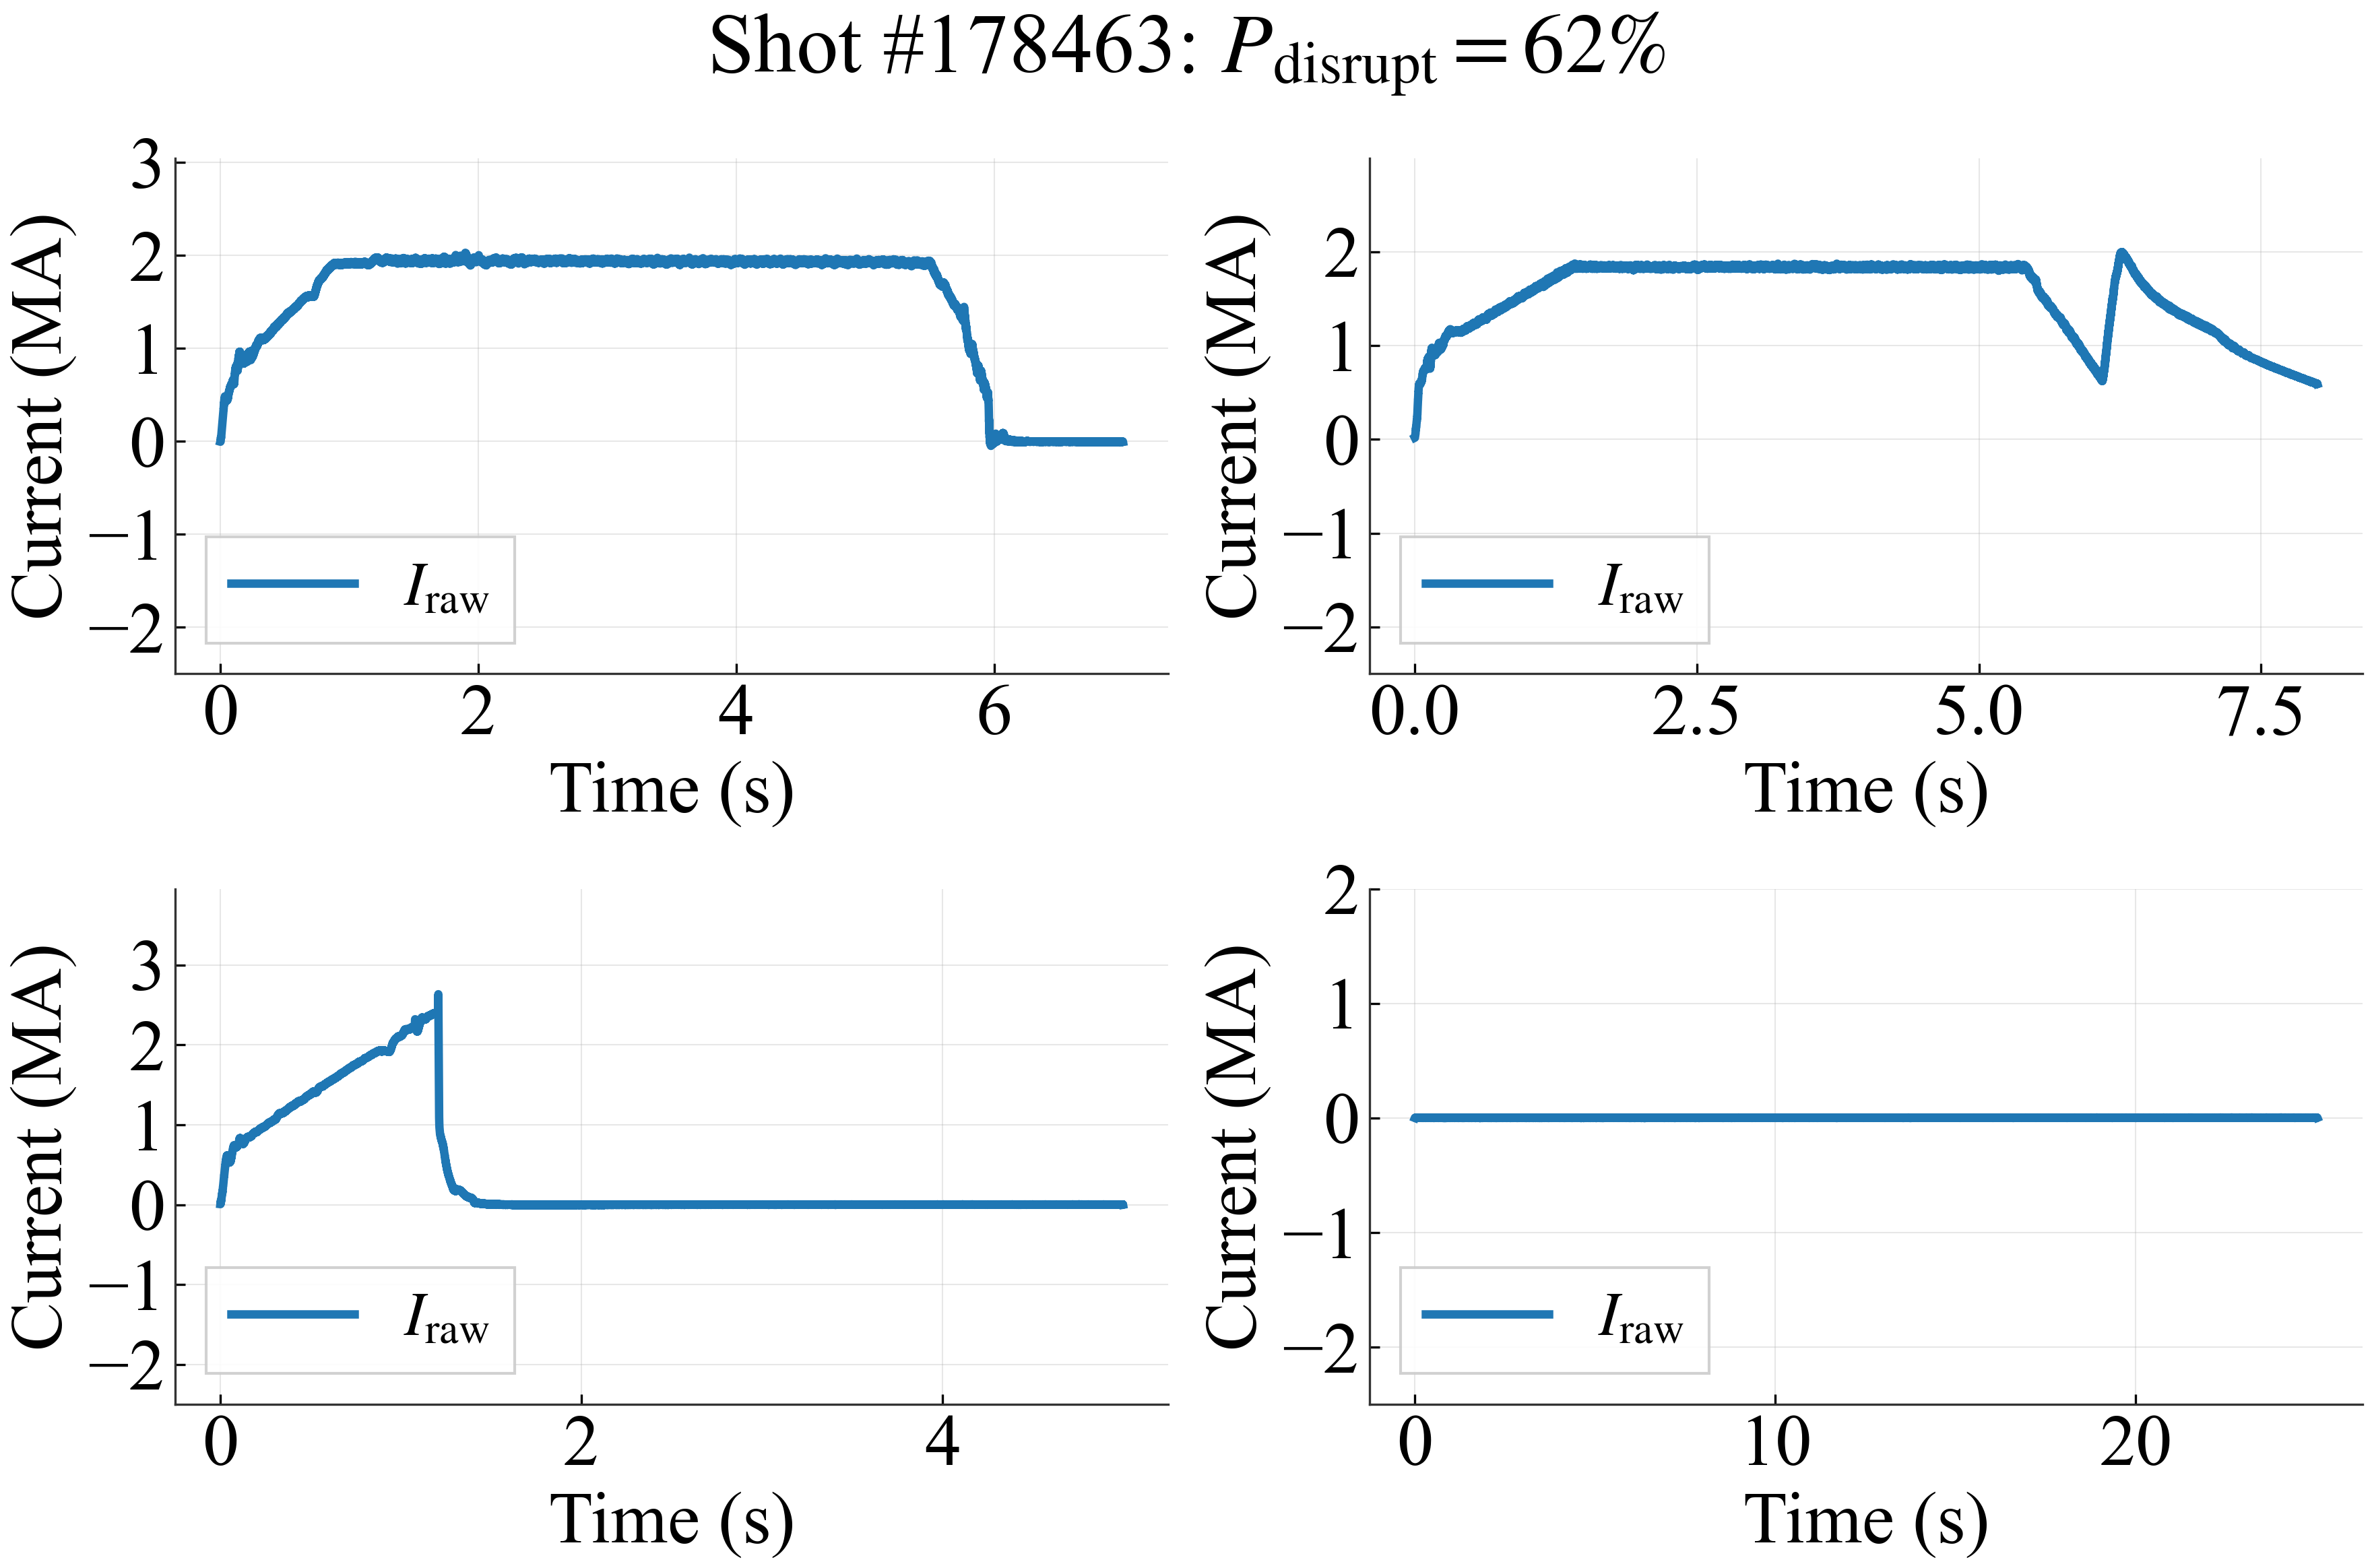
\includegraphics[width=\textwidth]{best_model/select_false_positives.png}
    \caption{Four selected non-disruptive shots incorrectly identified as disruptive by the CNN. Shots 178891 and 176423 have a drop that somewhat resembles a disruption, confusing the model. Notice that the CNN disruption probability is lower for the more confusing shots.}
    \label{sub:false_positives}
  \end{subfigure}

  \caption{Analysis of CNN classification errors for disruptive Figure~\ref{sub:false_negatives} and non-disruptive Figure~Figure~\ref{sub:false_positives} shots.}
  \label{fig:cnn_errors} 
\end{figure*}

\section{Convolutional Heuristic for Time of Disruption}

For any given shot, let the current be $I(t)$, $t\in[0, T]$. We start by noting that shots with $\max{I(t)}\approx0$ are negative polarity shots and must be flipped before proceeding (Eq~\eqref{raw_current}). 


\begin{equation}
  I_\mathrm{raw}(t) = \begin{cases}
    -I(t) & \max(I)\approx0 \\
    I(t) & \text{otherwise}
  \end{cases}
  \label{raw_current}
\end{equation}

We then calculate a smoothed current $I_\mathrm{smooth}(t)$ by applying a moving average convolution with a window size $K=T / S$, where $S=300$ is an experimentally determined smoothing parameter. The convolution of $I(t)$ with a function $g(t)$ is given by $g\ast f(t)=\int_{0}^{t}g(\tau)\,f(t-\tau)\,d\tau$; for a moving average, $g$ is a constant, simplifying our expression to Eq~\eqref{current_smooth}.

\begin{equation}
  \label{current_smooth}
  I_\mathrm{smooth}(t) = \frac{1}{K} \int_{t-K}^{t}I(\tau)\,d\tau
\end{equation}

Note that we compute the moving average on our dataset as a discrete convolution, applying \verb|np.convolve| on the current tensor Eq~\eqref {current_tensor}. The $i$th component of the smooth current $\mathbf{I}_\mathrm{smooth}$ is $\mathbf{I}_{\mathrm{smooth}_i} = \frac{1}{K} \sum_{k=1}^{K} I_{i-k}$.

We then define the time of disruption heuristic $f(t)$ as the difference between the raw $I(t)$ and smooth current Eq~\eqref{current_smooth}. 


\begin{equation}
  \label{heuristic}
  f(t)=I_\mathrm{raw}(t) - I_\mathrm{smooth}(t)
\end{equation}

To find the start $t=t_0$ of a disruption, we simply search for the global maximum of $f(t)$. The first local minimum of $f(t), \ t>t_0$ identifies the end of disruption $t_f$.


\begin{equation}
  \label{time_of_disrupt}
  t_0=\max(f(t))
\end{equation}

\

We apply this heuristic on our test holdout set, consisting of 3943 total shots, of which 889 are disruptive.

\begin{figure}[t]
  \centering
  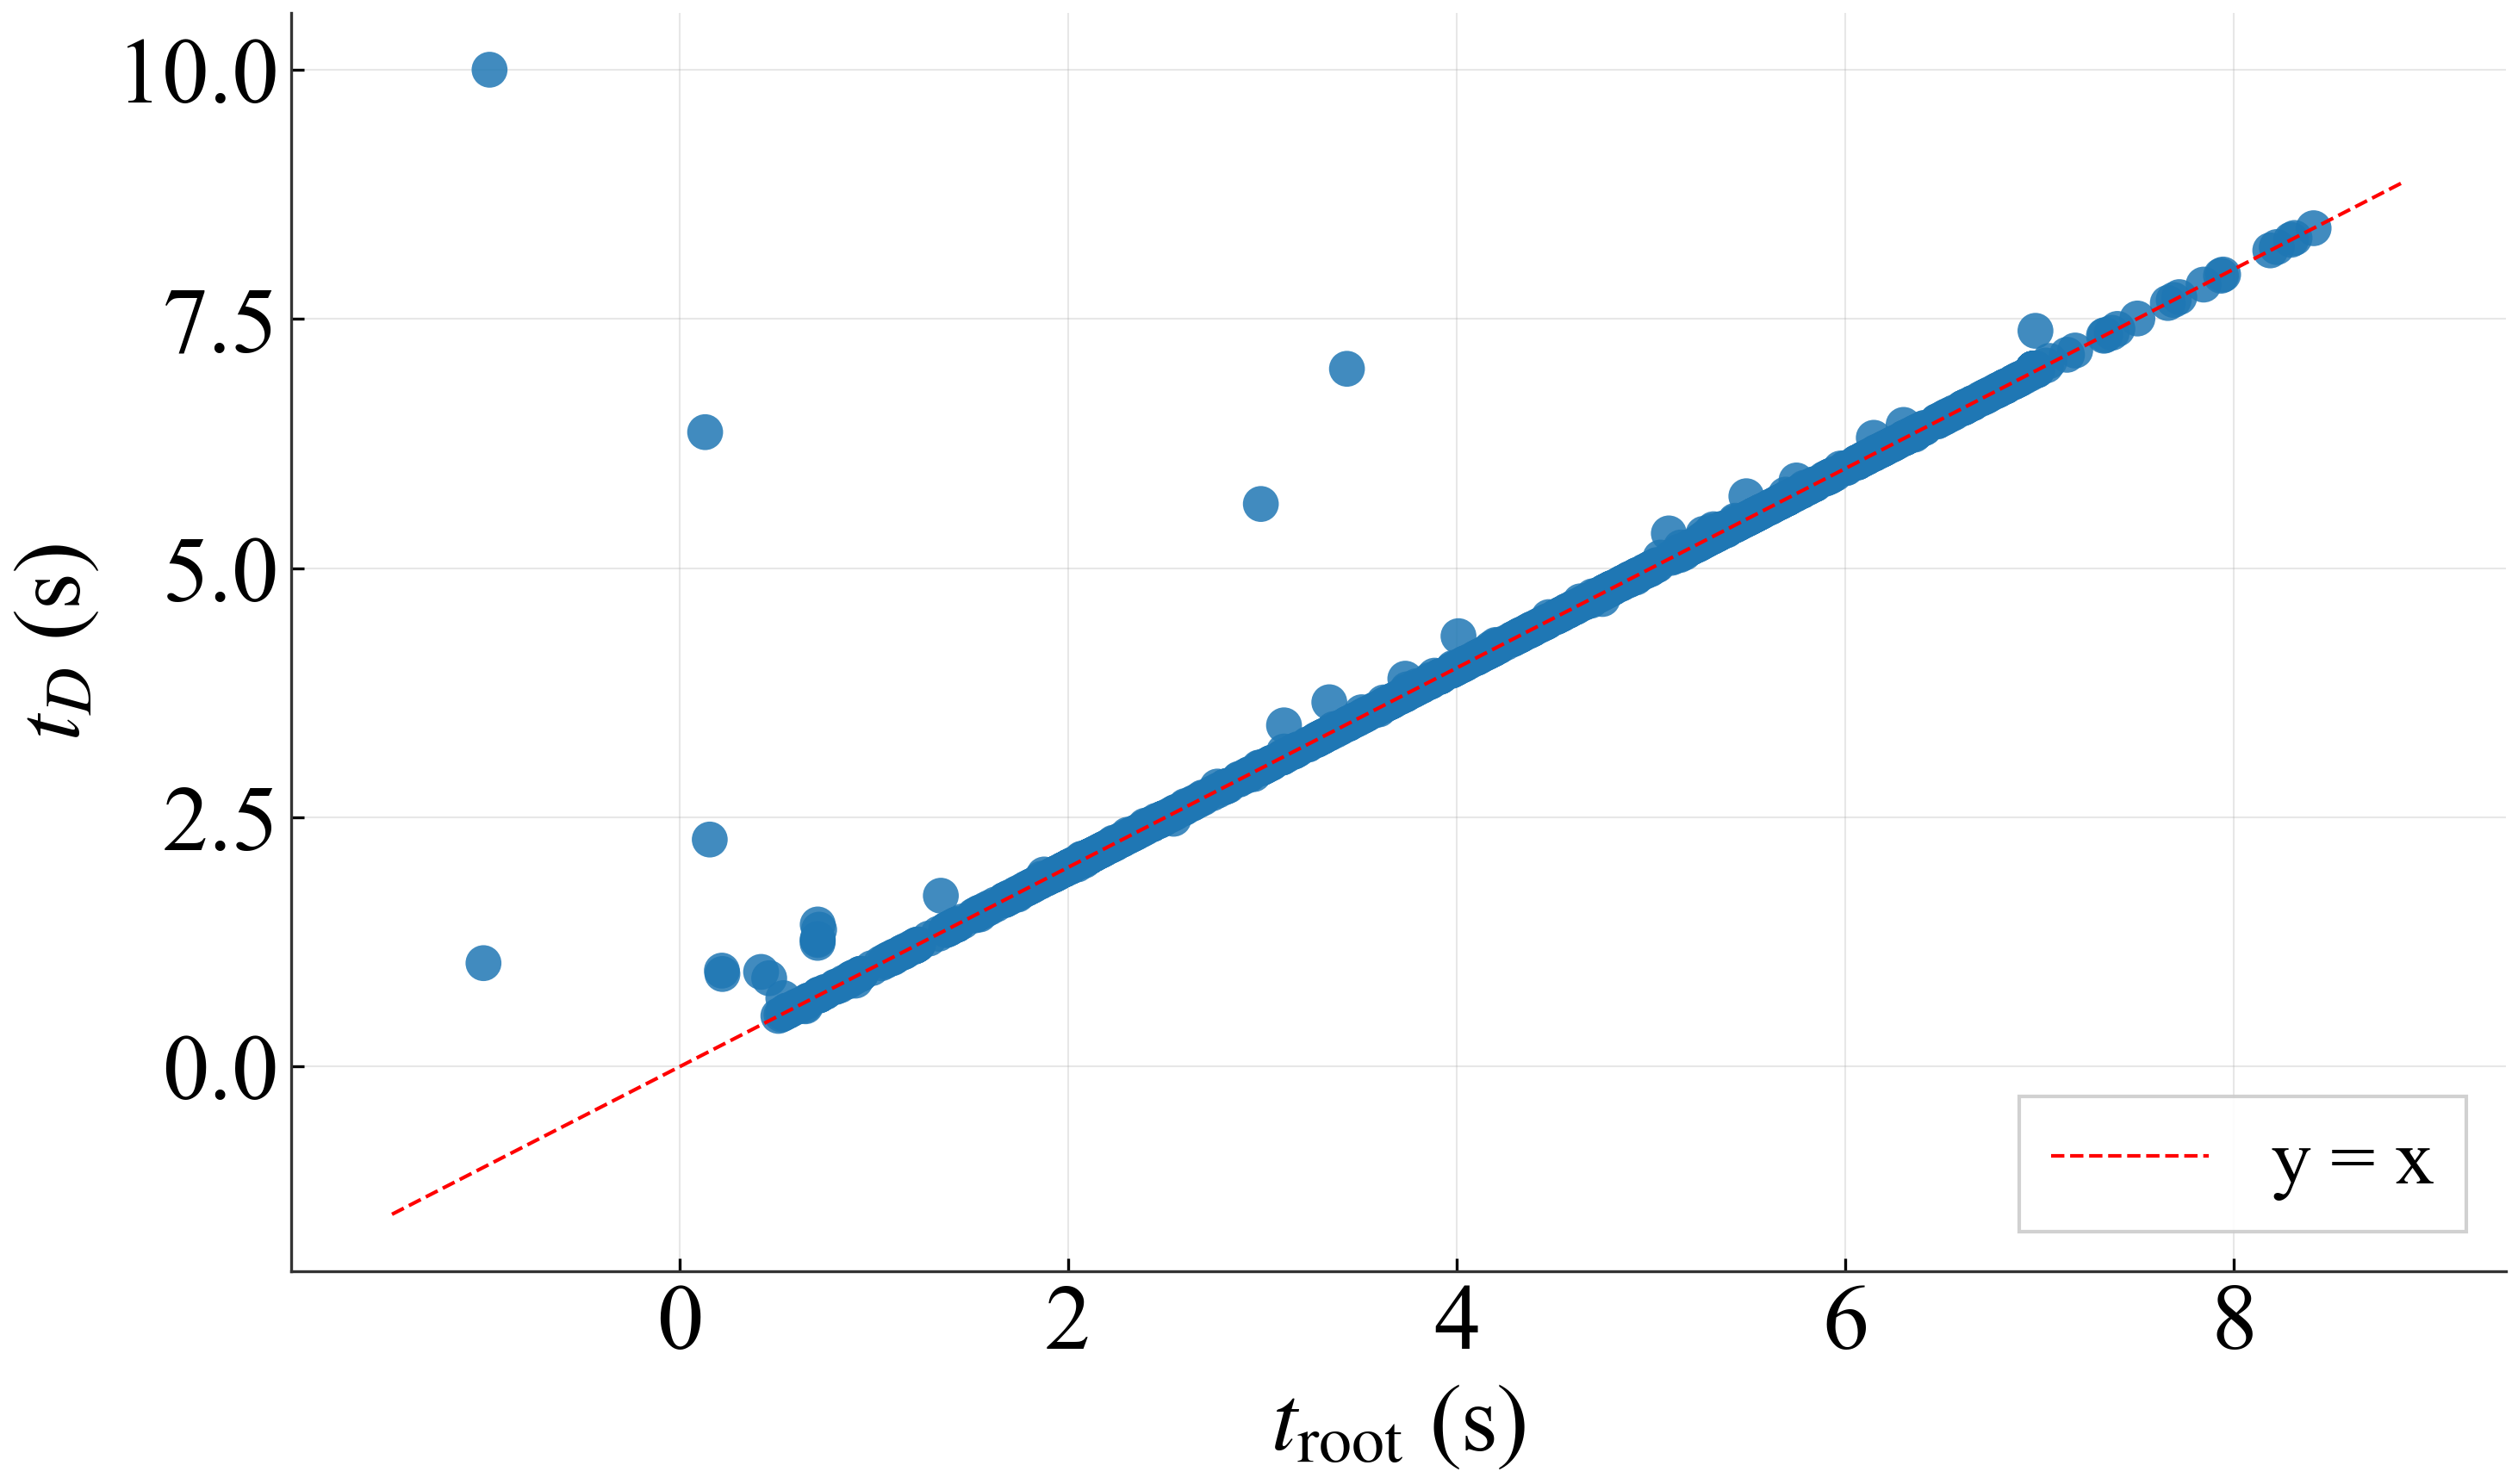
\includegraphics[width=1\columnwidth]{best_model/predictions_scatter_pred_root.png}
  \caption{Predicted disruption time Eq~\eqref{time_of_disrupt} vs real disruption time for 889 test holdout shots. We see a few outliers, with the majority of predictions on the accurate $y=x$ line.}
  \label{fig:predictions_scatter}
\end{figure}

Comparing $t_0$ to the labeled disruption times $\{t_D\}$ in our test set, we find that most of our predictions are early by $\Delta t = t_0-t_D \approx \qty{-4}{\milli\s}$ (Figure~\ref{sub/disruption_time_diff_start}). Therefore, we conclude that the DIII-D team labels shots mid-disruption, somewhere in the range $t_0\geq t \leq t_f$. If we use the first root $t_\mathrm{root}$ (Eq~\eqref{time_of_disrupt_root}) as the predicted disruption time, we get a more normalized distribution of $\Delta t = t_\mathrm{root}-t_D$ Figure~\ref{sub/disruption_time_diff_root}.

 \begin{equation}
  \label{time_of_disrupt_root}
  f(t_\mathrm{root})=0, \quad t_\mathrm{root}\in[t_0, t_f]
 \end{equation}
 

\begin{figure*}[htp]
  \centering
  
  \begin{subfigure}[b]{0.48\textwidth}
    \centering
    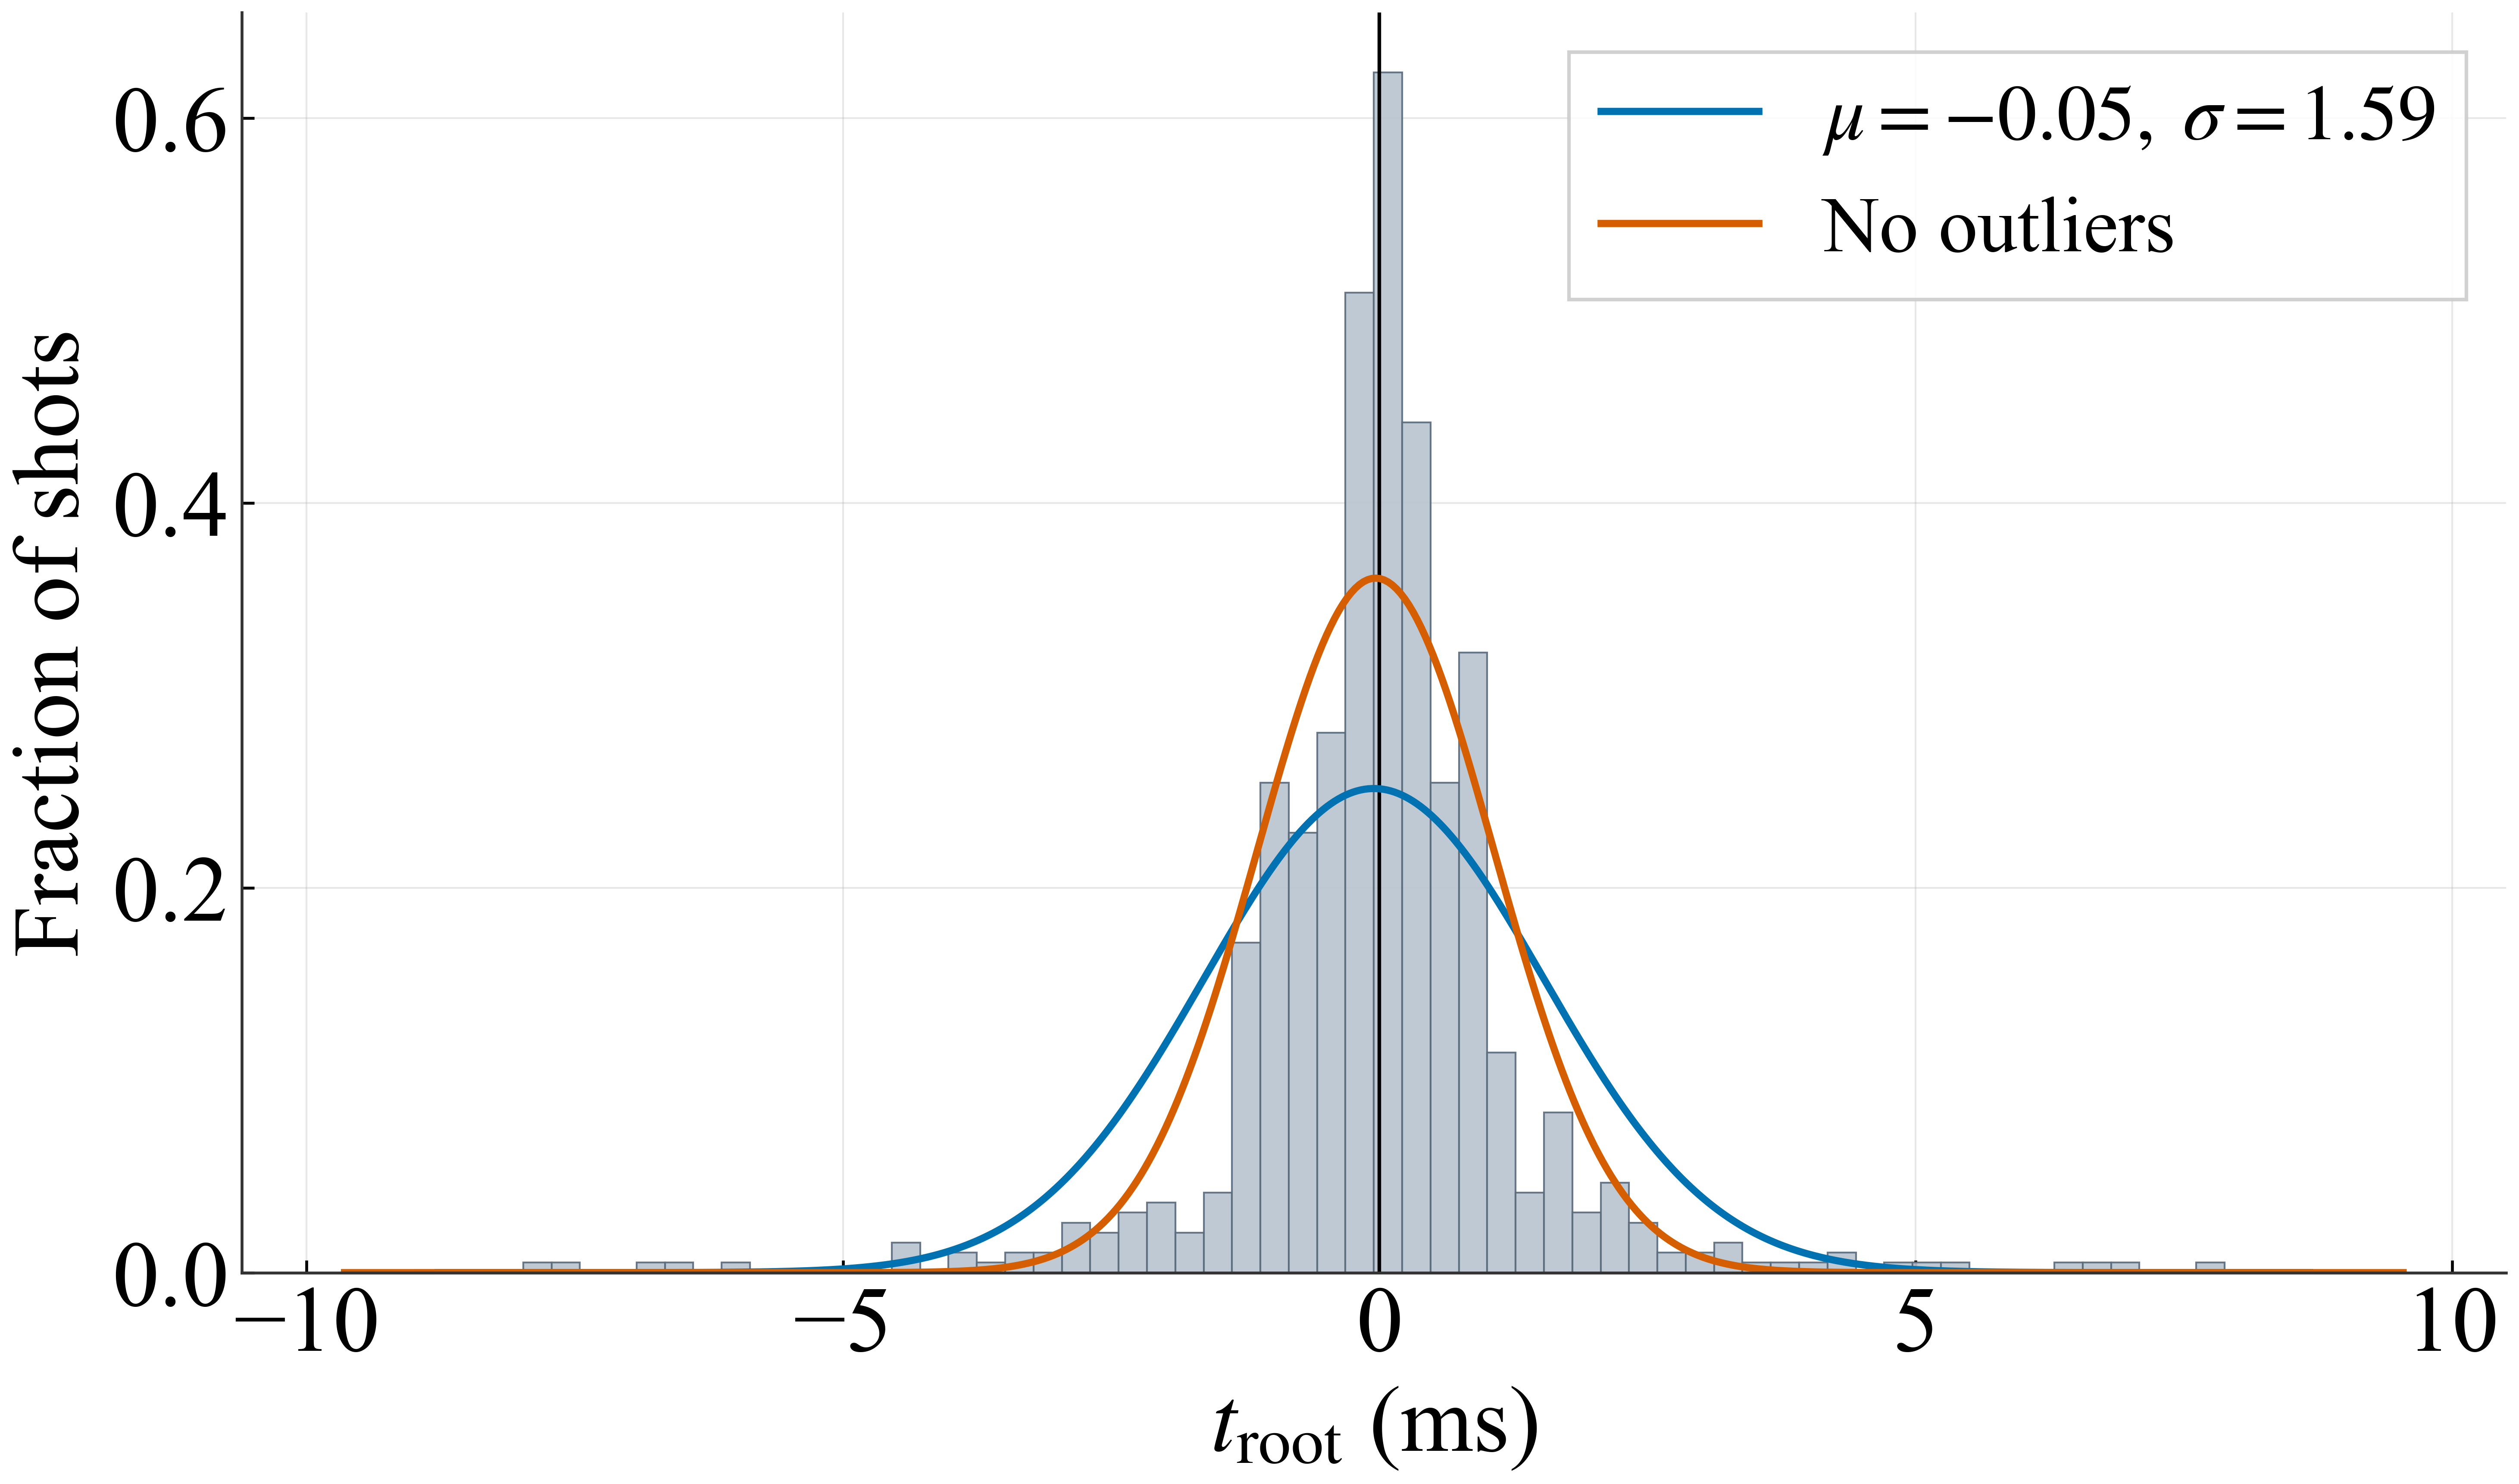
\includegraphics[width=\textwidth]{best_model/disruption_time_diff_pred_root.png}
    \caption{Histogram of the difference $\Delta t$ between heuristic root $t_\mathrm{root}$ Eq~\eqref{time_of_disrupt_root} and labeled time of disruption in milliseconds. The Gaussian is centered with $\mu\approx \qty{0}{\milli\s}$, $\sigma=\qty{1.1}{\milli\s}$}
    \label{sub/disruption_time_diff_root}
  \end{subfigure}
  \hfill
  \begin{subfigure}[b]{0.48\textwidth}
    \centering
    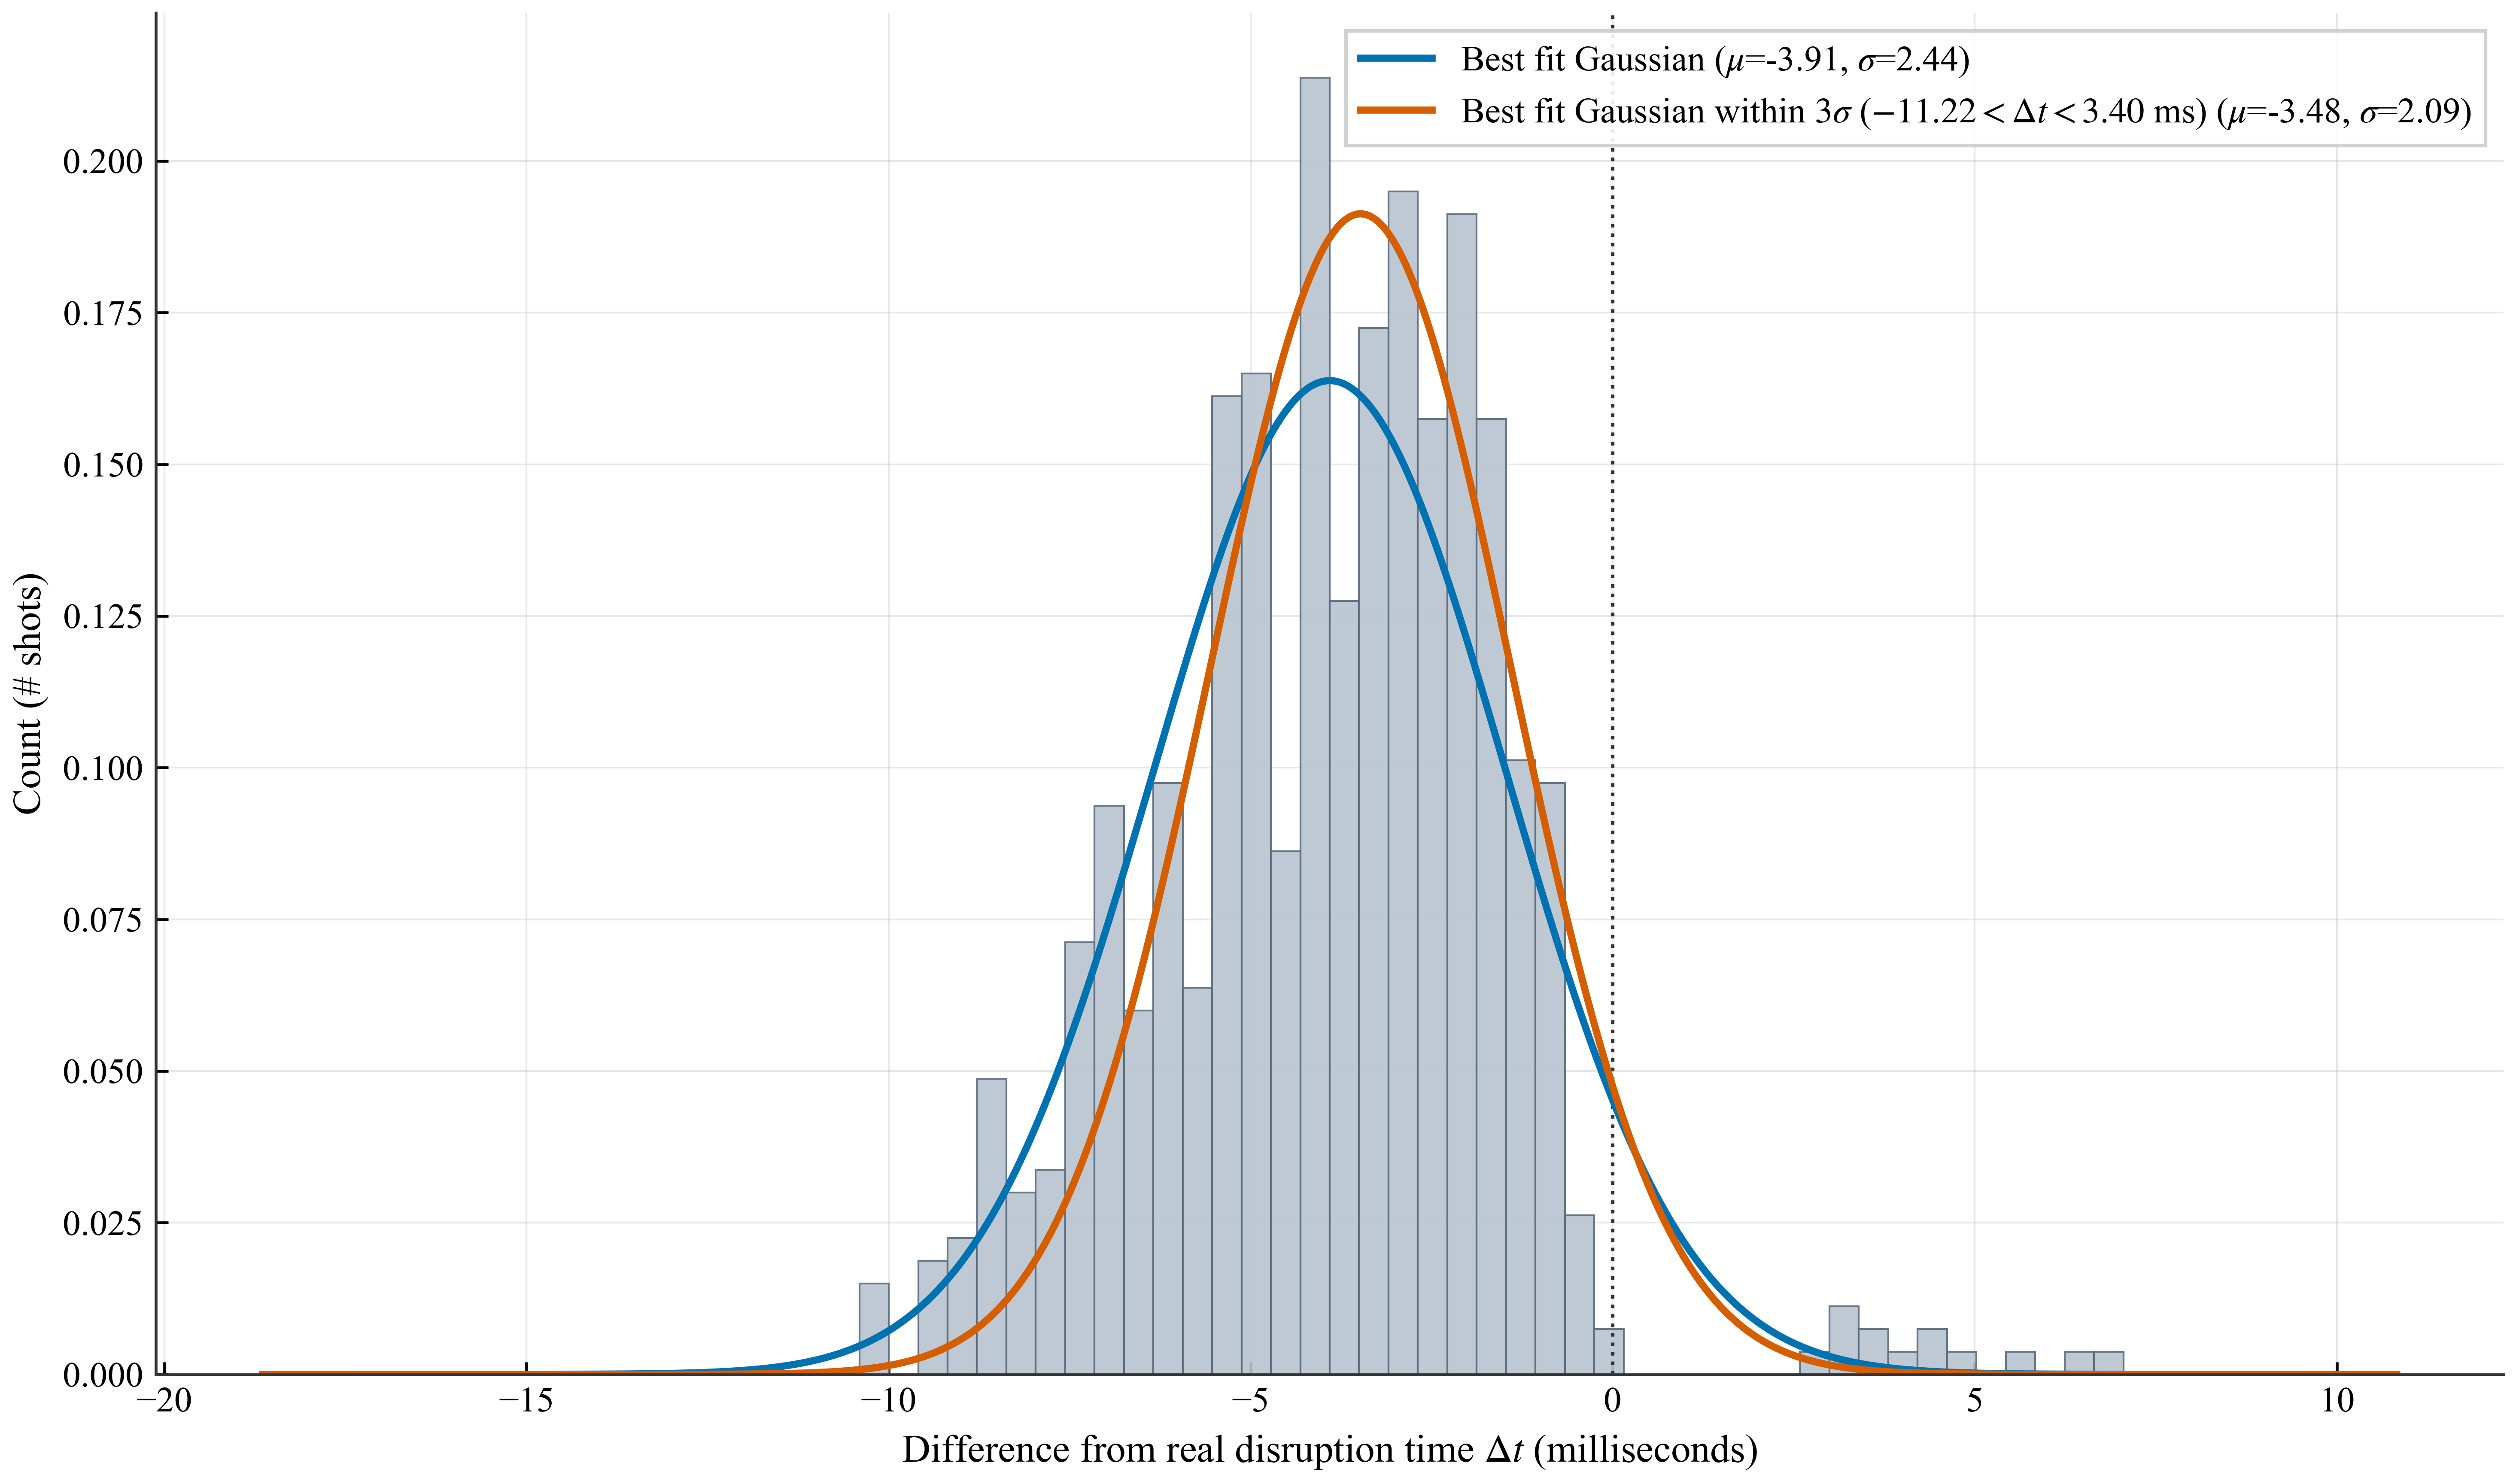
\includegraphics[width=\textwidth]{best_model/disruption_time_diff_pred_start.png}
    \caption{Histogram of the difference $\Delta t$ between predicted start of disruption Eq~\eqref{time_of_disrupt} and labeled time of disruption in milliseconds. Most of our predictions are early, with a mean $\Delta t \approx \qty{-4}{\milli\s}$}
    \label{sub:disruption_time_diff_start}
  \end{subfigure}

  \caption{Histogram of the predicted disruption time error $\Delta t$, using both the disruption start and disruption root.}
  \label{fig:heuristic_diff} 
\end{figure*}


% ==================================================================
\section{Conclusion}
\label{sec:conclusion}

We train a multi-layer Convolutional Neural Network to classify shots from the DIII-D Tokamak Reactor as disruptive/non-disruptive using 1-Dimensional current vs. time data. We use a $F_\beta=1.5$ performance metric to favor recall over precision and perform hyperparameter tuning over 100 trials; the trained classifier correctly identifies 99\% of disruptive shots on our test holdout set, producing less than 9\% false positives. We also develop a convolutional formula to identify the disruption time in disruptive shots with a median of $0$ and a standard deviation of $\qty{1}{\milli\s}$, with an option to additionally identify the full time-span of a disruption. Our algorithm can generate automated labeling of every DIII-D shot up to the current day, and should generalize well to other Tokamak reactors, providing a much larger labeled dataset to the scientific community for developing richer models.


\section*{Acknowledgments}
Our thanks to Argonne National Laboratory for providing us with the data to train our model. 

\section*{Data and code availability}
Code for the model, along with the best model weights and hyperparamters, are hosted at https://github.com/starlightjason2/DLDL.git. Cursor \cite{cursor2026} and Claude \cite{claude2026} were utilized for code development.

% ------------------------------------------------------------------
\bibliographystyle{unsrtnat}
\bibliography{references}

\end{document}
